\chapter{Problem statement and proposal}\label{B:problemStatementAndProposal}

As this title's chapter sample, the aim of this section is to provide a structured vision of the specific problems of each issue to be developed during this project.

Main issues are about to prepare and/or adapt current technologies to be ready for a cloud deployment. This fact implies studying existing technologies and tools in order to create specific microservices that will be interconnected between them. And, finally to carry out required developments in order to assure the goals behind and ease demonstrate the results.

\section{Architecture statement}

Therefore, above all it's required to define the platform's architecture to prototype in order to have a global and generic insight. So, taking into account the pieces required for this project (i.e.: service layer, monitoring layer, virtualization/deploy layer), such architecture should contain the different high level layers as shown next:
\begin{figure}[htb]
\begin{center}
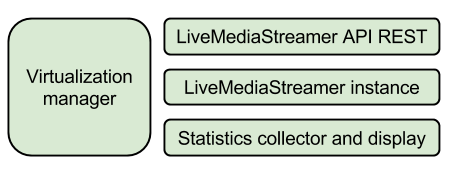
\includegraphics[width=0.6\textwidth]{./images/generalArch.png}
\caption{Generic platform architecture}
\label{F:genericPlatArch}
\end{center}
\end{figure}

The "LiveMediaStreamer REST API" layer will contain the service that will be offered to different and external applications (communicating over HTTP) in order to manage the "LiveMediaStreamer instance" layer by creating different audio and video production scenarios. Both layers are the core layers of the platform. 

Moreover, in order to offer a centralized monitoring system, the "Statistics collector and display" layer becomes as the generic box for this requirement.

Then, it is also required to provide an orchestrator that manages the deployment and distribution of the possible configurations for the previous introduced layers. This will be done thanks to the "Virtualization manager" layer.

Finally, to point out that how the communication between each layer is going to be carried out is treated in next chapters.

\subsection{Virtualization}

This subsection aims to introduce the possibilities that different virtualization technologies could offer for this project requirements and to decide between one of them.

First of all, next points are showing which are the expected outcomes for using virtualization and what should fulfil the selected technology:

\begin{itemize}
\item To manage and maintain a system of small pieces of services (assure a microservice architecture based pattern)
\item To have flexibility in order to quickly load (e.g.: start, restart, stop) required instances (e.g.: to assure real-time scalability) and to deploy any possible required scenario/configuration.
\item To offer ease to continuous develop and deploy the different parts of the architecture
\item To have version like system for having different version tags for the architecture modules (e.g.: a development and a production box of the same REST API service)
\item To assure full compatibility for the core layers' operating system (right now only Linux environments are supported)
\item To assure full compatibility for the hardware to work with (mainly x86 processors are in the scope)
\end{itemize}

Moreover, it is also required to use an as much lightweight as possible technology, and this fact is also because of this project aims to virtualize each piece of the platform architecture.

Under Linux environments there are many virtualization options (most of them proprietary) to analyse, but lets focus on the ones that are open-source and have wider and active communities behind.

These are KVM with QEMU and LXC with Docker:

\begin{itemize}
\item KVM (Kernel-based Virtual Machines) \hfill

It's a FreeBSD and Linux kernel module that offers a full virtualization solution for Linux on x86 hardware containing virtualization extensions (Intel VT or AMD-V). It consists of a loadable kernel module that provides the core virtualization infrastructure and a processor specific module.
Usually, KVM runs with the QEMU (Quick Emulator) which is a complete and standalone emulating suite that performs hardware virtualization.

KVM with QEMU is able to offer virtualization for x86, PowerPC, and S/390 guests. For instance, when the target architecture is the same as the host architecture, QEMU can make use of KVM particular features in order to do not emulate CPU nor memory.

\begin{figure}[!htb]
\begin{center}
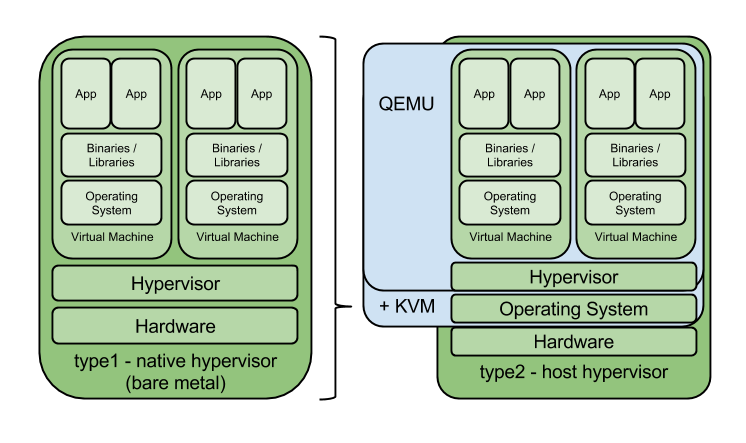
\includegraphics[width=0.9\textwidth]{./images/KVM.png}
\caption{QEMU with KVM or hypervisor type2 to type1}
\label{F:KVMandQEMU}
\end{center}
\end{figure}

Figure \ref{F:KVMandQEMU} showcases how KVM can convert a type2 hypervisor (i.e.: QEMU) into a type1 hypervisor (known as a bare metal hypervisor) which increases overall application performances. 

\item LXC (Linux Containers) \hfill

It's an operating-system-level virtualization environment for running multiple isolated Linux systems (known as containers) on a single Linux central host.

Linux kernel itself provides the cgroups functionality that allows limitation and prioritization of resources (CPU, memory, block I/O, network, etc.) without the need for starting any virtual machines, and namespace isolation functionality that allows complete isolation of an applications' view of the operating environment, including process trees, networking, user IDs and mounted file systems.

Nowadays virtualization tendencies are focusing on the Docker project, which is a platform that provides an additional layer of abstraction and automation of operating-system-level virtualization on Linux, Mac OS and Windows.
\begin{figure}[!htb]
\begin{center}
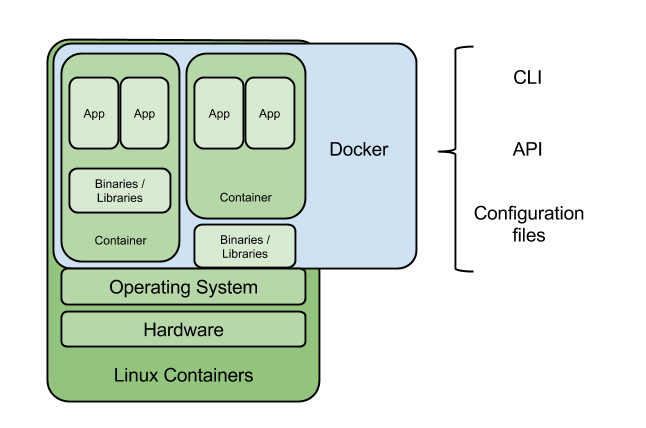
\includegraphics[width=0.9\textwidth]{./images/LXC.png}
\caption{Docker with LXC}
\label{F:DockerAndLXC}
\end{center}
\end{figure}

LXC with Docker mean resource isolation features of the Linux kernel to allow independent containers to run within a single Linux instance, avoiding the overhead of starting and maintaining virtual machines. Moreover, Docker project automates the deployment of applications inside software containers and offers different tools to manage them (i.e.: CLI, API and file configurations), as shown in figure \ref{F:DockerAndLXC} 
\end{itemize}

Thus, it seems that the technology that best suits this project requirements is the Docker project. Main reasons are the capabilities of ease maintain, test and quickly deploy each container. Moreover, ---APPENDIX X--- demonstrates that the performance offered in front of the Virtual Machine (i.e.: QEMU + KVM) one is rather better.

Finally, it's important to point out that another keypoint of the Docker solution is that lets intercommunicate containers that are in the same physical server without exposing network layer. This means much more security and performance over other virtualization solutions (at least of the simplicity point of view when intercommunicating instances).

\subsection{Monitoring layer}

Monitoring layer section aims to provide an insight of what are the minimum requirements for what monitoring is required in this project and which are the available tools of interest.

Following the same criteria as this project tends to, the tools that are going to be focused on are the ones that have an open-source philosophy behind. So, most of the tools and services around the Internet are directly ruled out.

As done in the virtualization problem statement section, it is required to showcase main requirements for the monitoring layer implementation:

\begin{itemize}
\item To ease its networkability.
\item To offer full control for specific configuration requirements and to not depend on external/enterprise services. To be fully deployable.
\item To be as lightweight as possible in terms of:
\begin{itemize}
\item Processing capacity
\item Memory utilization
\item Network throughput
\end{itemize}
\item To fit into a microservice architecture pattern.
\item To be supported under a Linux environment.
\item To offer much more capabilities than the required for future requirements (this is a requirement because this platform development is supposed to be continued after this project)
\item To support RRD (Round Robin Database) as a DBMS (Database Management System) in order to assure data storage size from the beginning.
\end{itemize}

Next list to showcase takes into account the data that should be gathered:

\begin{itemize}
\item CPU and memory usage per process which is part of the platform.
\item Network usage (per process involved and per media)
\item Internal core service performance parameters (i.e.: LiveMediaStreamer core performance):
\begin{itemize}
\item Processing time
\item Losses ratio
\end{itemize}
\end{itemize}

Moreover, in order to be fitted into a microservices pattern, it's required to split the monitoring layer. The proposal, as usually done in many monitoring systems is as follows:
\begin{itemize}
\item Gathering layer \hfill

It only will be responsible of the gathering, distribution and storing of the metrics.

\item Display layer

It only will be responsible of the data display as a function of user-specific queries.

\end{itemize}
To point out that a possible alert layer is treated as a future work because it becomes out of scope. The main reason is that this project is focused on measuring and demonstrating that such platform is feasible, next steps would be to compose a set of alarms and actuators system in order to become as automated as possible.

Once previous steps have been shown, it's time to analyse technologies of interest in order to decide between one of them.

So, the following list shows some of the analysed tools that might fit project's requirement as previously exposed:

\begin{itemize}
\item Munin \hfill

Cross-platform web-based network monitoring and graphing tool designed as a front-end application. Written in Perl.

\item RRDTool \hfill

Known as an industry standard, high performance data logging and graphing system for time series data. Written in C and runs under GNU/Linux, Windows and AIX platforms.

\item Collectd \hfill

Small daemon which collects system information periodically and provides mechanisms to store and monitor the values in a variety of ways. Written in C and support any unix-like O.S.

\item Graphite \hfill

Tool for monitoring and graphing the performance of computer systems, which collects, stores, and displays time series data in real time.

\end{itemize}

Many other solutions have been discarded due to depend on specific enterprises' roadmap or due to not fit under previously exposed requirements. (REFERENCE Comparison of network monitoring systems WIKIPEDIA) 

Finally, Collectd and Graphite are the selected tools. Main reasons are due to being fully configurable and its core design and philosophy. Collectd has a data distribution system based on a push model and it can be single deployed (i.e.: gathering and display layer), but it is going to be used with the storage and display tool Graphite. This fact is due to assure high performance for the containers where the Collectd will be gathering and transmitting metrics through UDP, and because of both tools lead to create a microservice architecture monitoring layer. Moreover, Graphite software will be deployed as a centralized storing and displaying tool which will be feed from many Collectds. Another reason to select Collectd is due to being fully compatible with Docker (Collectd can be deployed inside a container and there is also an official plugin to monitor Docker containers in an O.S.). 

Finally, Graphite has also been selected because it offers a HTTP API which ease its scalability. 

So, the monitoring layer is proposed to be designed as shown next:

\begin{figure}[htb]
\begin{center}
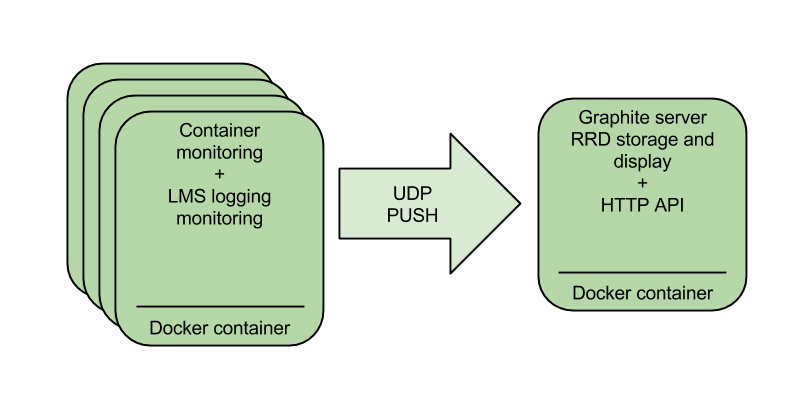
\includegraphics[width=0.9\textwidth]{./images/mlap.png}
\caption{Monitoring layer architecture proposal}
\label{F:MLAP}
\end{center}
\end{figure}

\subsection{Application layer}\label{B:appLayerCH2}

This subsection aims to compile the minimum requirements that the core service (i.e.: the LiveMediaStreamer framework) should implement to fit within the platform. This means assuring that it can be demonstrated as an efficient real-time cloud production platform, as a prototype.

First of all, let's showcase main topics application's (i.e.: LiveMediaStreamer framework) developments should take into account:

\begin{itemize}
	\item To assure minimal performance (i.e.: computational) cost when measuring internal metrics in order to not take effect on the overall performance of the framework, whatever the scenario setup
	\item To calculate specific metrics of interest. Common metrics should be:
	\begin{itemize}
		\item For network usage statistics
		\begin{itemize}
			\item Bandwidth usage per incoming and outgoing streams
			\item Packet losses per per incoming and outgoing streams
			\item Jitter per incoming and outgoing streams
			\item Delay per incoming and outgoing streams
		\end{itemize}
		\item For media statistics
		\begin{itemize}
			\item Frame losses (to measure how many frames are lost at each filter)
			\item Pipeline delay (to measure the overall time a frame is processed inside pipeline). It could be said as "Frame processing time" too. 
		\end{itemize}
	\end{itemize}
	\item To compile the metrics in an efficient manner in order to let them be gathered for Collectd or any other application.
\end{itemize}

Current LiveMediaStreamer framework's version does not implement any metrics gathering neither logging.

Regarding network usage statistics, current LiveMediaStreamer's version does not support any internal metrics gathering at network modules (i.e.: receiver and transmitter) where the Live555 library is implemented. However, Live555 library lend to quickly implement network statistics measurements (i.e.: bandwidth, losses, jitter, delay). 

Thanks to Live555 examples (i.e.: the testProgs folder inside the source code library path) it becomes easy to understand how to gather network statistics at input side. But, regarding output network statistics, it is not so obvious which is the optimal solution. This fact is mainly due to having two options which imply to implement the metrics gathering by doing some methods' re-implementation of the RTP or the RTCP main classes, but this specific problem statement will be treated at chapter 5 ANCHOR CHAPTER 5.

Regarding media statistics, current LiveMediaStreamers' version of the framework does not implement any metrics gathering. So, in order to minimize computational cost of such measurements what is proposed to implement is shown next:

\begin{itemize}
\item To implement specific method to measure processing delays.
\item To implement specific method to measure frame losses.
\end{itemize}

Then, a main issue have to be taken into account regarding how to implement the metrics presentations in order to let them be logged for external applications. This is regarding current middleware API, which is not at all an API but a web GUI API for an specific scenario (i.e.: AVMixer scenario, as said in state of the art's chapter \ref{SOA:LMSframework}), which means that it is required to implement a more generic middleware API to let external applications to log the LMS internal metrics as API (--REFERENCE--) definition reclaims. 

Therefore, the proposal for this issue is to develop a RESTfull API in order to present the metrics from the LMS instance. This implementation is an opportunity to develop a full API for managing the LiveMediaStreamer framework over HTTP.  Moreover, such middleware will ease to develop new applications over the LMS framework by evolving it as a SaaS, which means a proper enhancement to fit in a cloud environment. 

\begin{figure}[htb]
\begin{center}
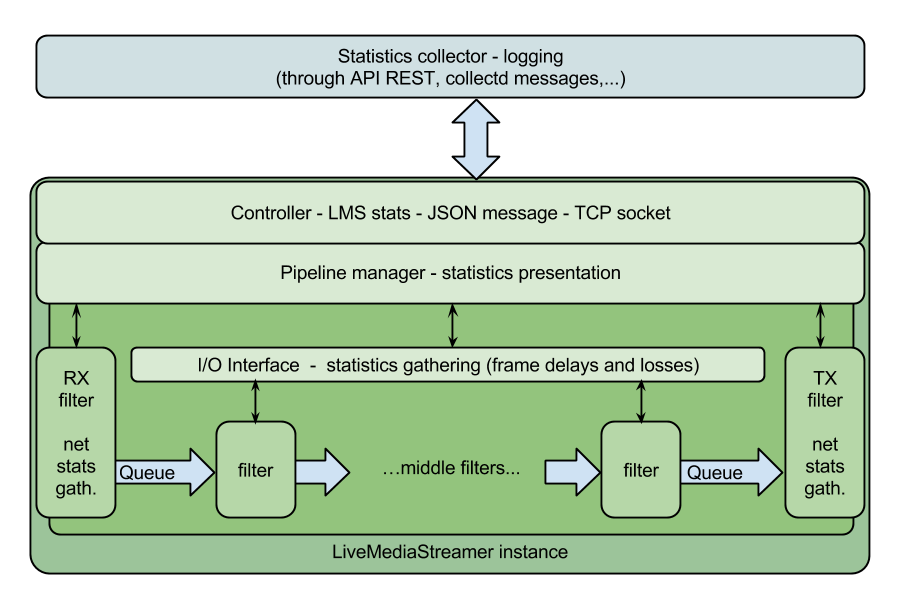
\includegraphics[width=0.95\textwidth]{./images/appArch.png}
\caption{LiveMediaStreamer framework statistics gathering and logging proposal}
\label{F:appArch}
\end{center}
\end{figure}

Figure \ref{F:appArch} showcases how previous statements are proposed to be implemented. As it can be seen in APPENDIX \ref{ANX:lmsarchfull}, each filter can have one or more readers and writers (both are inheritors of the IOInterface class) and concretely at the reader level there is the optimal point to detect frame losses and processing delays. This means measuring from the last writer (i.e.: a queue and the filter itself) when flushing frames (when the frame is supposed to be ready). Therefore, this fact implies having the chance to measure the delays at time-stamp level and the lost frames at sequence number level. But this will be developed in chapter \ref{D:application}.

On the other hand, the Pipelinemanager class instance is the responsible class to compile the metrics filter by filter when they are requested by the Controller class instance. 

\section{Architecture proposal}

Once the problem statement has been focused per each defined layer (i.e.: virtualization, monitoring and application) of the platform, an overall architecture can be proposed. This is shown in figure \ref{F:overallArchProp}.

\begin{figure}[!htb]
\begin{center}
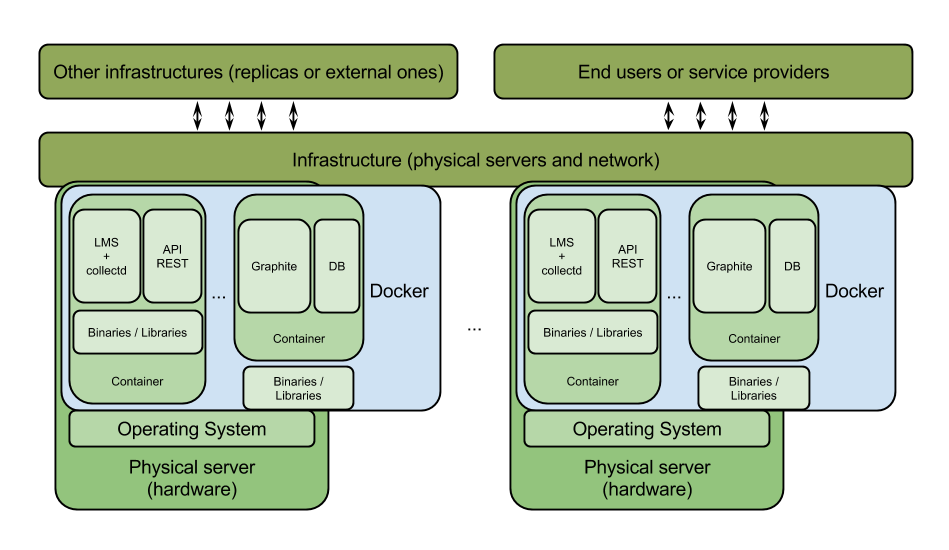
\includegraphics[width=0.95\textwidth]{./images/overallArchProp.png}
\caption{Proposal of the platform architecture}
\label{F:overallArchProp}
\end{center}
\end{figure}

Figure \ref{F:overallArchProp} tries to be as generic as possible in order to showcase the possibilities of the platform. As seen, there are different physical servers presented in order to demonstrate the aim to also support flexibility and scalability. However, following chapters (concretely the conclusions chapter \ref{H:platformDeploymentAndDemonstrations}) will demonstrate if it is feasible. 
Moreover, each physical server has different types of containers where are shown different and possible combinations and configurations of the technologies that might be deployed and used for specific use cases (scenarios).

For example, a possible and specific architecture configuration could be a transcoder scenario:

\begin{figure}[!htb]
\begin{center}
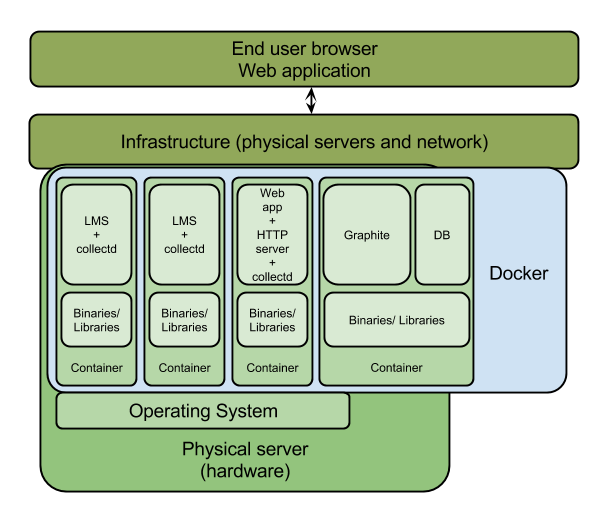
\includegraphics[width=0.7\textwidth]{./images/exampleArch.png}
\caption{Example of specific platform deployment}
\label{F:exampleArch}
\end{center}
\end{figure}

Figure \ref{F:exampleArch} is a simple example of a transcoding servicde behind a web application. This use case example takes into account an user, which configures and manages the LiveMediaStreamer's scenario configured for a transcoding service (e.g.: starting with a HTML input form for incoming inputs, transcoding parameters and RTSP server configuration). Concretely, at architecture level, there is a container with an LMS daemon running, another one with the REST API that receives queries from the HTTP server from another container, which is serving the web application to the end user, which is using the application through a web browser. Then, each container has a collectd client that parses the logs of interest and it sends the metrics to the Graphite service running. Therefore, at the web application the user could be able to see specific graphics (e.g.: CPU usage, lost frames, bandwidth usage, \ldots) from the graphite server (in another container) in order to monitor the overall performance and actuate if required. Finally, to point out that this scenario could be splitted into different O.S.. 

Finally, to point out that what will be deployed in order to demonstrate the platform feasibility is an specific but as generic as possible scenario. However, this topic will be treated in chapter \ref{H:platformDeploymentAndDemonstrations}.


\section{Task planning}

Finally, this last section aims to organize the tasks to be done in terms of developments. 

\begin{figure}[!htb]
\begin{center}
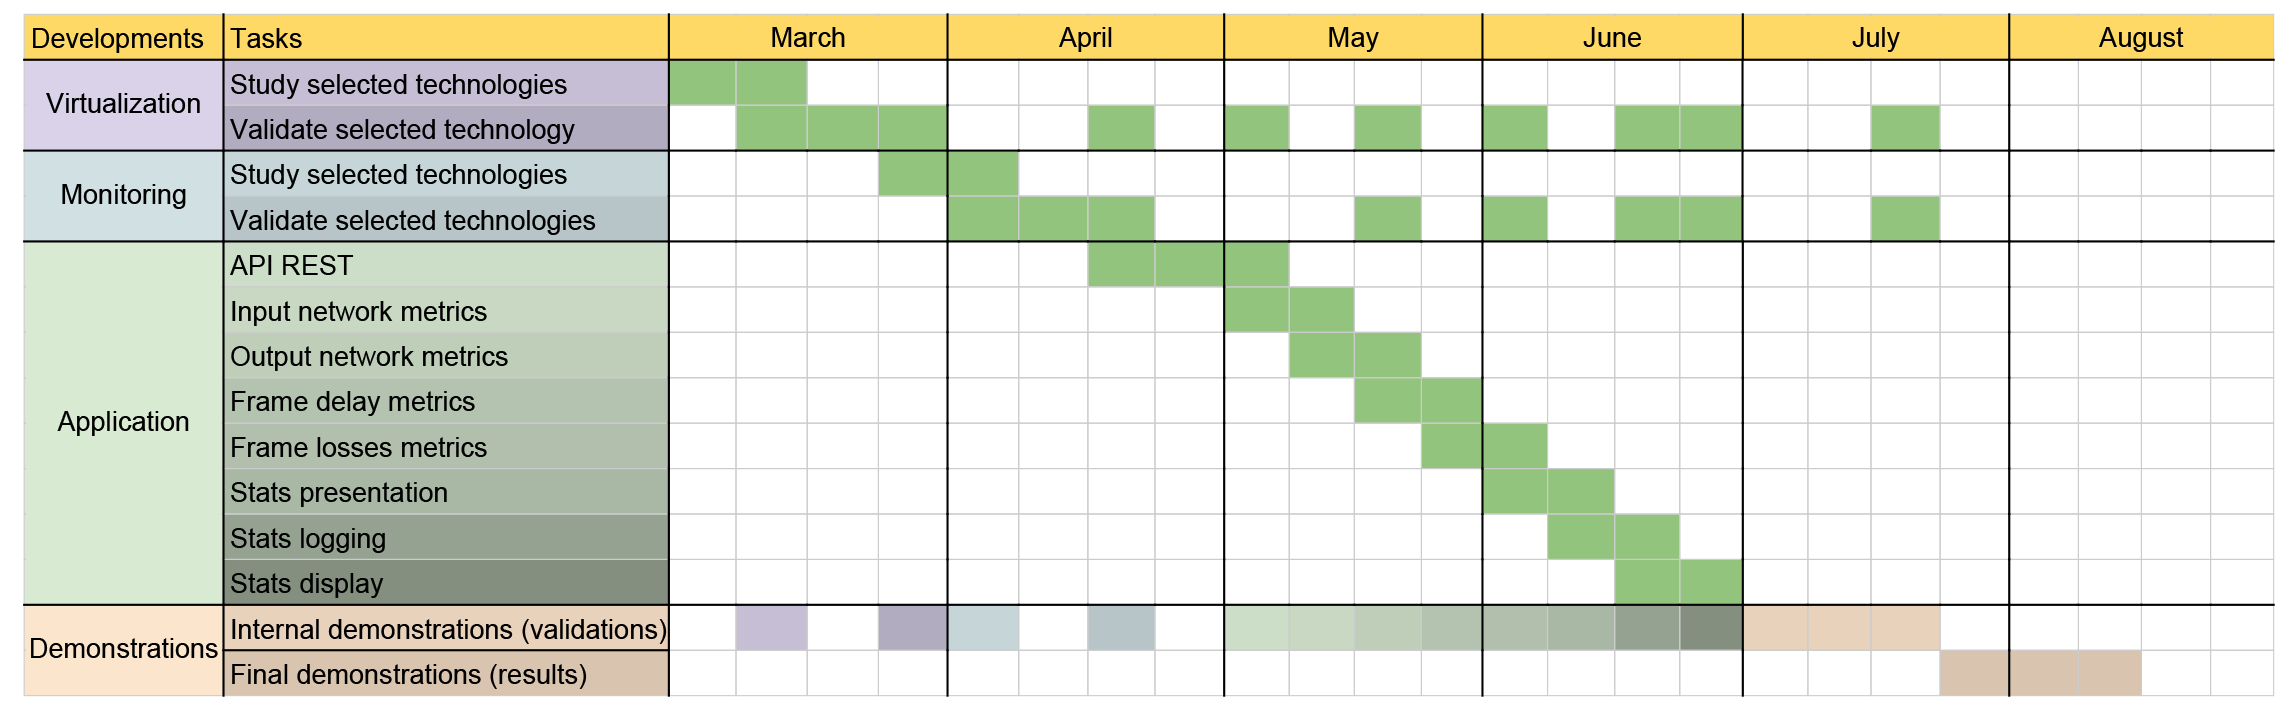
\includegraphics[width=1\textwidth]{./images/gantt.png}
\caption{Task planning - Gantt proposal}
\label{F:tpgp}
\end{center}
\end{figure}

Figure \ref{F:tpgp} is the Gantt proposal for the task planning organization. It takes into account the period of six months for the project and is showing specific periods per task when they should be executed, as a reference. For example, some tasks might seem overloaded about time, but this is taking into account that the whole time I'm not going to be working on the project but other tasks related to my job position at the i2CAT Foundation.

Finally, to point out that the fact of being working with a team and behind an organization, it is important to take into account internal demonstrations periods in order to carry out specific validations. This is due to reach an agreement between the team, because the intention is to take profit of this project.

Next chapters aims to showcase the work done per each topic developed. These are application (chapter \ref{D:application}), monitoring (chapter \ref{G:monitoringLayer}), virtualization chapter \ref{D:virtualization}) and final deployment demonstrations (chapter \ref{H:platformDeploymentAndDemonstrations}). 
